

\chapter{Sistema de controlo e monitorização}


Este capítulo tem como objetivo a descrição do sistema que resultou do trabalho prático
desta dissertação. Para esse fim, cada elemento pertencente ao sistema é caracterizado de
acordo com as suas funções e especificidades. É também descrito como os elementos interagem
entre si.

A figura 4.1 representa o diagrama de blocos do sistema, onde se encontram todos os seus
elementos, seguidamente descritos.




Tendo como base, por um lado os resultados da pesquisa efectuada em 2003 e, por outro lado, as
indicações e expectativas fornecidas pelos representantes da Liftech, empresa que actua neste
projecto como o cliente do produto a desenvolver, foi elaborada a especificação funcional do
sistema.
Neste capítulo são descritos separadamente cada um dos módulos que compõem o sistema, quer
ao nível da sua arquitectura, quer ao nível do software de suporte.


\section{Descrição global do sistema}



Este sistema tem como objectivo a supervisão remota de elevadores, permitindo não só a
monitorização e registo de eventos, como também a actuação remota de comandos e o registo de
assistências técnicas.


\begin{figure}[!htb]
	\centering
	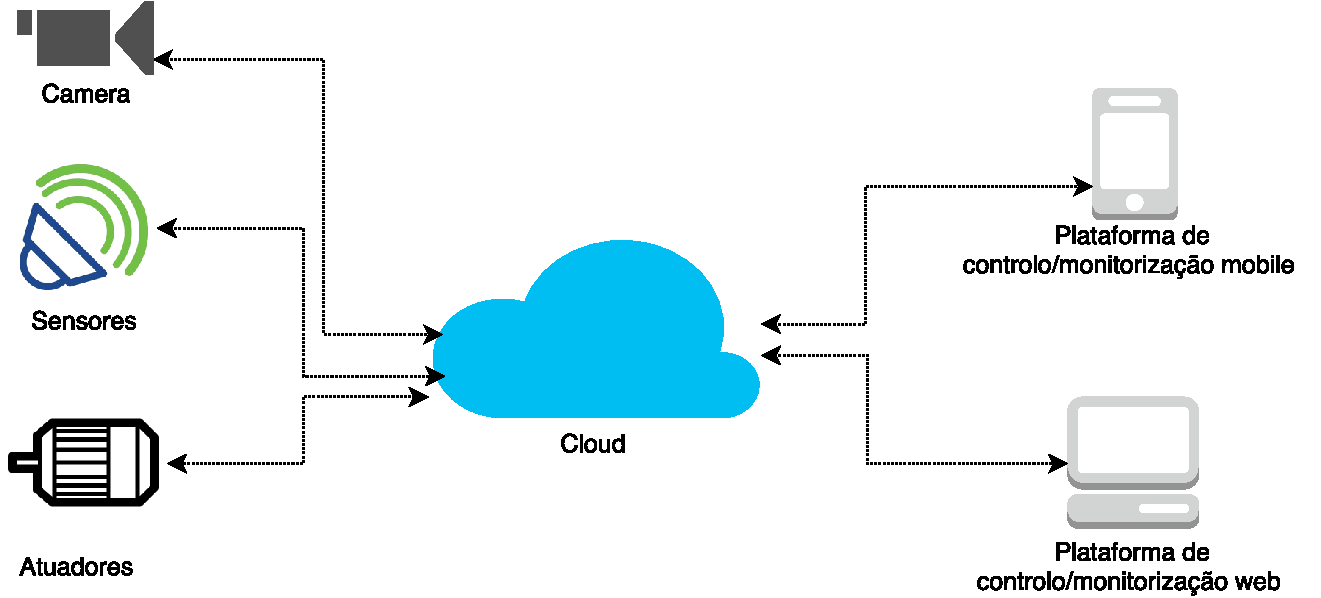
\includegraphics[scale=0.45]{esquemas/global_arquitetura.pdf}
	\caption{Ilustração de uma "quinta" onde se produz salicornia}
	\label{dikw}
\end{figure}







Como vimos no capitulo 3, uma plantação de  salicórnia carece de um controlo relativamente fino da salinidade do terreno onde ela cresce. A salinidade do terreno depende, por sua vez, das chuvas, da salinidade da água dos canais da ria, etc. Nas “quintas” de salicórnia da Ria, a produção faz-se numa espécie de leiras limitadas por pequenos canais de irrigação. Esses canais podem ser cheios de água salgada proveniente dos esteiros que rodeiam a “quinta”. Essa operação implica a abertura de válvulas de admissão dessa água, medida do nível da maré nos canais, monitorização da qualidade e salinidade da água exterior.
Por sua vez, a cultura pode ser ameaçada por excesso de água doce de chuvas ou ser objeto de vandalismo.





Neste contexto, cada grupo de sensores espalhado por cada leira irá comunicar com um módulo central. Por sua vez, este módulo irá comunicar diretamente com a servidor que possibilitará que os dados sejam tratados e disponíveis para visualização. Pressupõe-se portanto que este ultimo módulo tenha necessariamente ligação à rede wifi de modo a conseguir consumir a API rest que se pretende desenvolver. 


\section{Componentes}

Durante esta dissertação é necessário reter dois conceitos principais: 

\begin{itemize}
	\item \textbf{\textit{Sensor Module }(SM):} microcontrolador responsável pela aquisição de dados provenientes dos mais diversos tipos de sensores. Cada \textit{sensor module} terá que utilizar um determinado modulo de comunicação de modo a possibilitar a comunicação com o módulo central. 
	 
	\item \textbf{\textit{Controller Module }(CM):} microcontrolador responsável pela recepção dos dados preveniente dos \textit{sensor models} 
\end{itemize}







\begin{figure}[!htb]
	\centering
	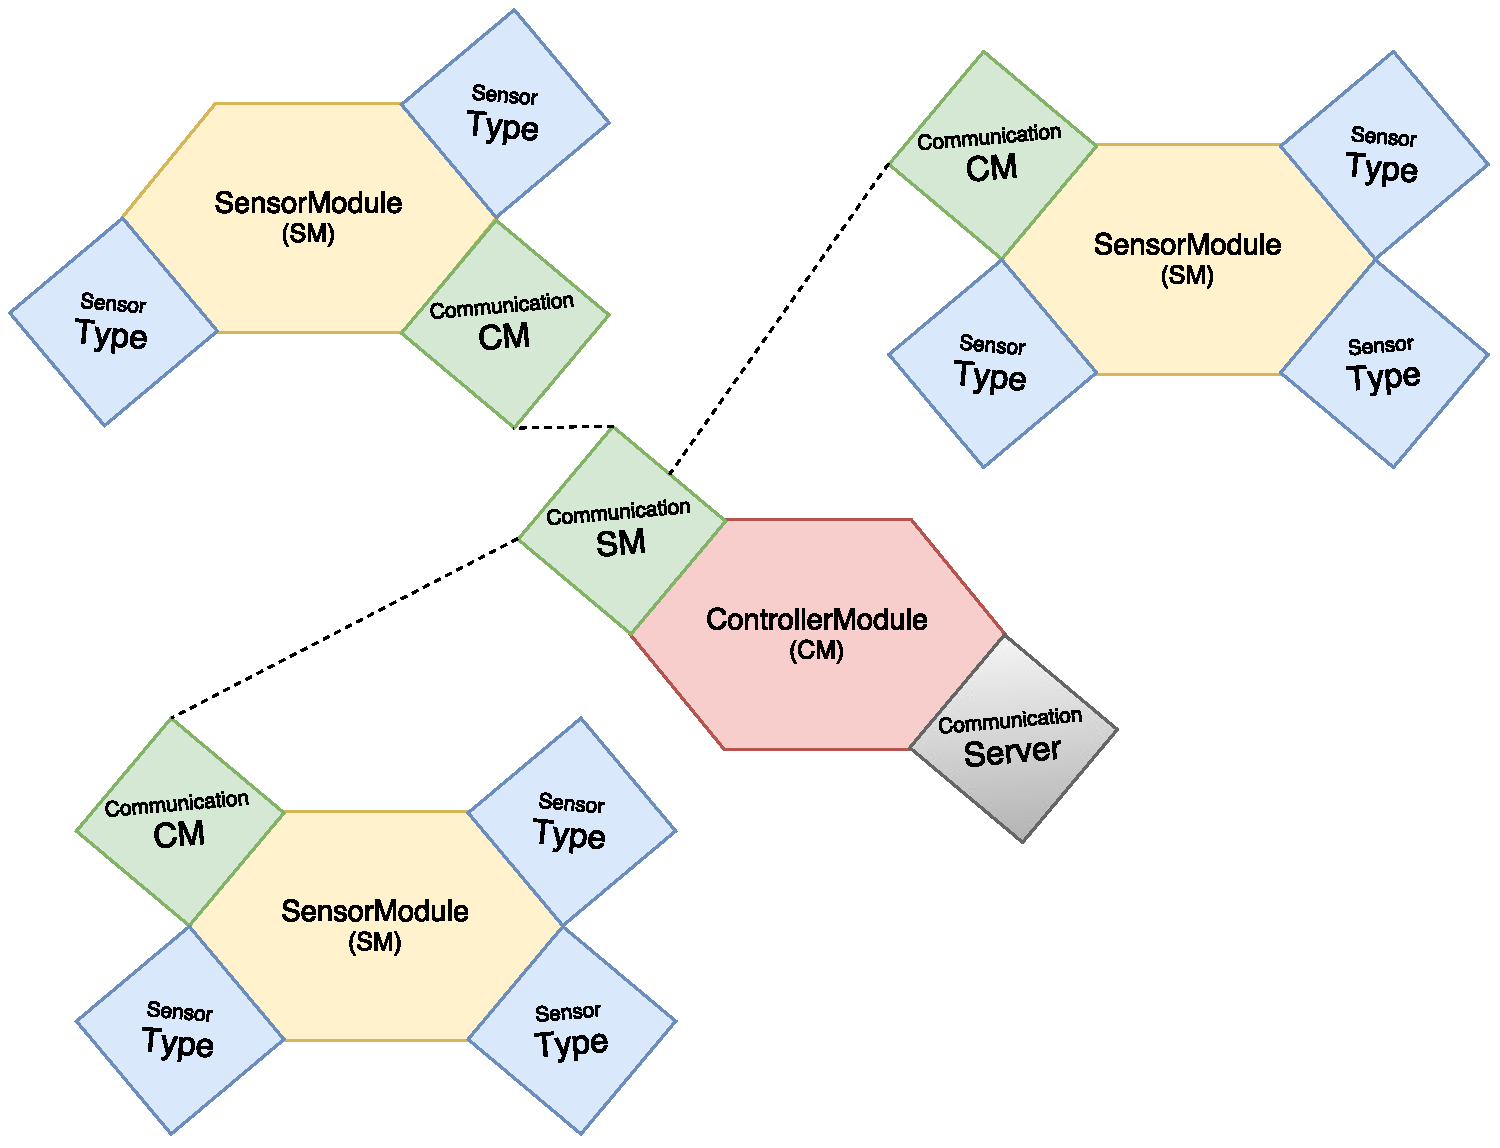
\includegraphics[scale=0.45]{esquemas/general-electronic-modules.pdf}
	\caption{Pirâmide do conhecimento: modelo DIKW}
	\label{dikw}
\end{figure}








\newpage

\begin{figure}[!htb]
	\centering
	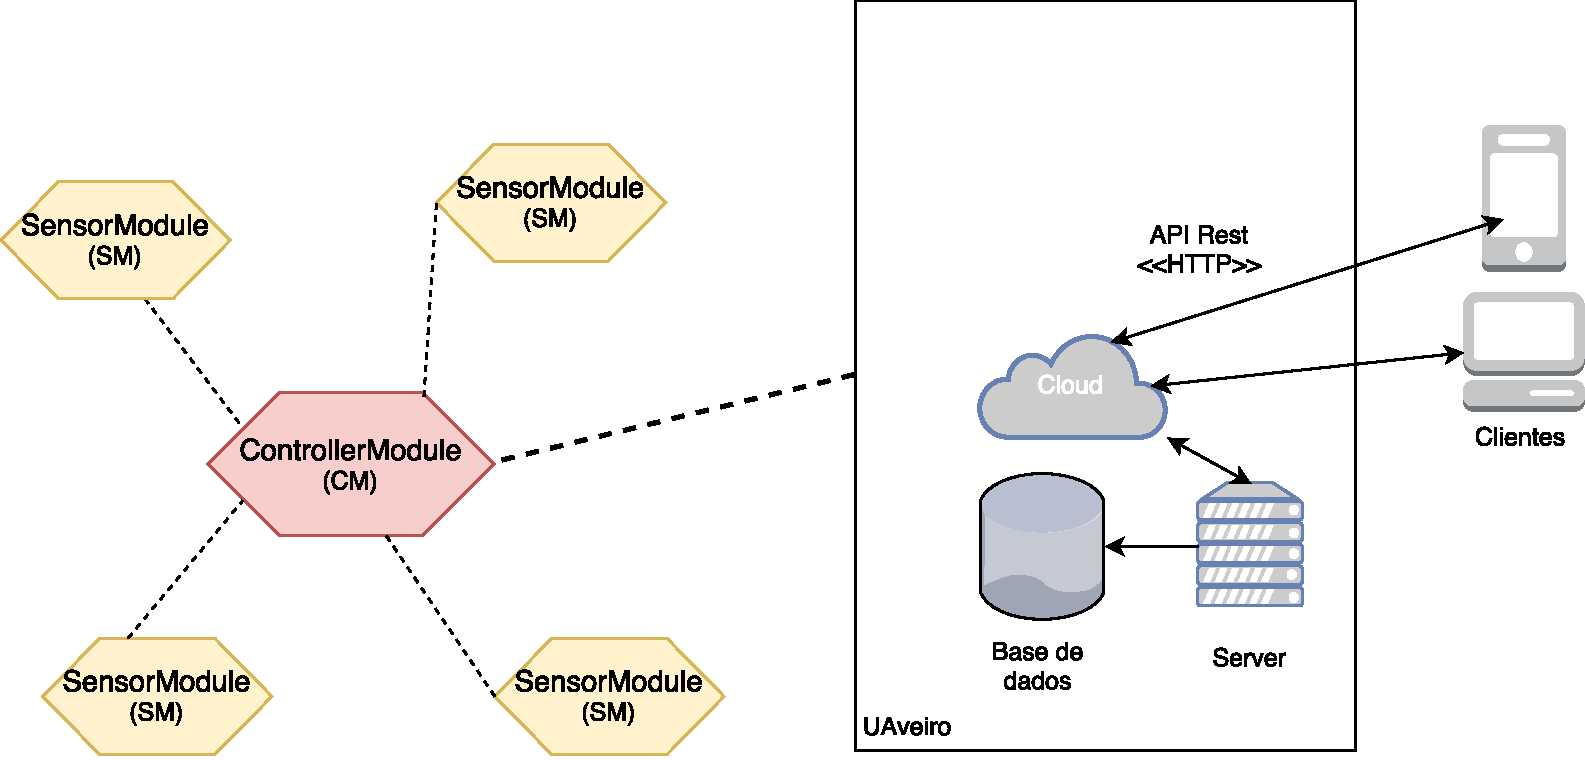
\includegraphics[scale=0.55]{esquemas/arquitetura_geral.pdf}
	\caption{Pirâmide do conhecimento: modelo DIKW}
	\label{dikw}
\end{figure}




\section{Design funcional}











\subsection{Requisitos funcionais}


%Os requisitos funcionais especificam os critérios que devem ser usados ​​para avaliar comportamentos ou funções especificas do sistema. Estes são os requisitos funcionais do sistema proposto nesta dissertação. 


A interface do sistema deve permitir que o usuário faça login no sistema
Admin ou um usuário.


A interface do sistema deve permitir que o usuário saia do sistema.



O sistema deve permitir o armazenamento de informações do cliente.


O sistema deve permitir a atualização das informações do cliente.


\subsection{Requisitos não funcionais}







\section{Design técnico}



\subsection{Arquitetura do sistema}



\subsubsection{Camada de apresentação}


\subsubsection{Camada de negócio}



\subsubsection{Camada de dados}




\section{Diagrama de componentes}




\section{Sistema de interação}


\section{Descrição}


Modulos da daniela : Cc1110



\section{Arquitetura geral}




\newpage












\section{Considerações finais}